
# 1. Introduction

  

建筑施工作业具有较高的安全与健康风险。美国劳工统计局报告，2024 年建筑与开采职业发生 1,032 起致命工伤 `\refjump{bls2024}{1}`{=tex}。除事故伤害外，混凝土、砂浆等含硅材料相关作业还可能造成可吸入结晶二氧化硅暴露，长期暴露与矽肺、肺癌和慢性阻塞性肺疾病等严重职业病有关 `\refjump{niosh2024}{2}`{=tex}。在混凝土地面施工中，整平和抹平又具有作业面积大、重复次数多、时间窗口受混凝土凝结过程约束等特点；人工施工需要长时间保持高体力负荷和重复动作，作业质量则依赖工人的经验、操作时机和熟练程度 `\refjump{albers2004}{3}`{=tex}, `\refjump{kobayashi1996}{4}`{=tex}。因此，将工人从重复、繁重且具有职业风险的地面作业中解放出来，同时提高表面质量的一致性，是建筑机器人研究中具有直接工程与社会价值的问题。

  

地面抹平机器人为这一问题提供了可行的机械化途径。已有现场试验表明，早期遥控抹平机器人能够完成从木抹到金属抹的多个工序，在 5 个工地累计作业约 1,000 m²，并在特定试验条件下达到约 317 m²/h 的平均作业能力 [4]。此后，研究者进一步在骑乘式抹光机上引入电动执行、激光定位、任务规划与远程监控，使机器人能够在预先给定的地面范围内自主行驶 [5]。近年来，摆臂式构型因其在保持紧凑车体的同时扩大末端抹盘工作范围而受到关注：相较于抹盘固定在车体前方或下方的普通抹平机器人，摆臂机器人可以在车体远离墙体、立柱和孔洞的情况下把圆形抹盘送至侧向或局部受限区域，使车体通行路径和末端作业轨迹部分解耦。这种构型有利于减少湿混凝土上的无效行驶和急转弯，并为边角、窄通道入口和障碍物附近的作业提供更大的姿态选择空间 [6]。

  

```{=tex}
\begin{figure}[H]
  \centering
  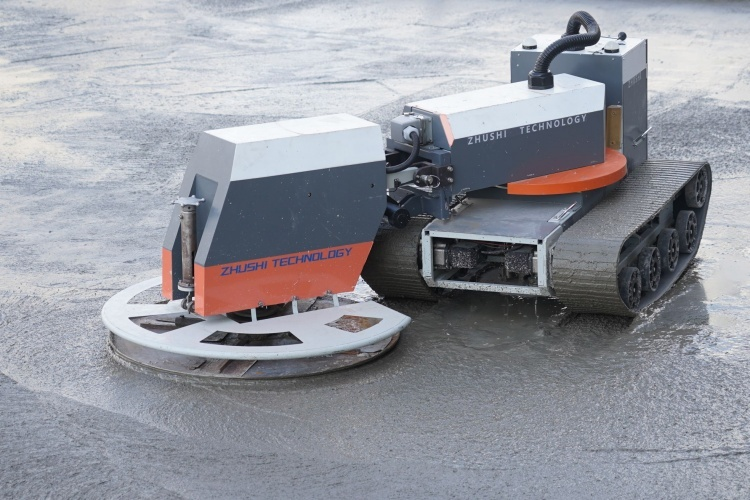
\includegraphics[width=0.78\linewidth]{figures/figure_1_swing_arm_troweling_robot_photo.jpg}
  \caption{摆臂式抹平机器人现场作业实拍。图中可见履带车体、摆臂/执行机构与末端圆形抹盘。图片来源：\href{https://sghexport.shobserver.com/html/toutiao/2021/08/13/511398.html}{上观新闻}，中建八局供图。}
\end{figure}
```

  

然而，机械化和遥控并不等同于自主化。人工遥控虽然能使操作者离开设备附近的危险区域，但仍要求操作者持续观察机器人和地面状态，并同时控制行驶、转向与抹平动作。其结果是，大面积作业中的漏抹、重复抹平、转弯痕迹和无效移动仍取决于人的判断；当墙体、立柱、预埋件和孔洞造成视线遮挡或通道破碎时，操作负担会进一步增加。早期现场试验也指出，突然转向可能留下轮迹、设备难以覆盖立柱和模板附近区域，且若干问题仍依赖操作者经验解决 [4]。现有摆臂机器人同样常采用人机协作或预定义轨迹，而非针对复杂场景自动生成完整作业路线 [6]。因此，若没有自主覆盖规划，机器人只是把体力劳动转化为持续的遥控与路径决策，作业质量和效率仍难以稳定复现。

  

从行业应用看，抹平机器人的工程价值已经通过现场样机和局部自主系统得到验证，但其进一步使用并不只取决于单机能否完成抹平动作。2024 年的一项承包商调查指出，机器人技术在受调查建筑企业中尚未实现广泛采用 [7]；对于混凝土地面作业而言，阻碍应用深化的关键环节之一，是机器人能否在真实施工平面中稳定处理墙体、立柱、预留孔洞和临时边界共同造成的复杂空间。已有系统已经展示了遥控抹平、规则区域内自主行驶或摆臂机器人可作业区域识别能力 [4–6]，但这些能力尚未自然转化为“给定一张含障碍施工地图即可输出完整、连续、可执行覆盖轨迹”的通用流程。因此，本文关注的不是单纯提高设备机械化程度，而是补全从施工地图和摆臂机器人几何到自主覆盖作业轨迹之间的规划链条。

  

这一任务本质上属于覆盖路径规划（Coverage Path Planning, CPP）：机器人需要在避开障碍的前提下，使作业工具扫过全部目标区域，并控制漏覆盖、重复覆盖、转场距离和总作业时间 [8]。但摆臂式抹平机器人的 CPP 不能直接套用传统的固定作业宽度模型。规划器不仅要决定车体经过哪里，还要决定摆臂如何运动、局部区域以何种顺序访问，以及圆形抹盘是否真正扫过目标地面。机器人状态至少包括车体位置、车体航向与摆臂角度，

  

$$
q=(x_c,y_c,\theta,\phi).
$$

  

随着 $\phi$ 变化，抹盘相对车体持续移动；实际覆盖是车体与摆臂共同形成的时变扫掠几何，而不是沿车体轨迹外扩一个固定宽度。摆臂的优势由此也成为规划难点：增大的可达范围可使车体远离墙体、立柱和孔洞，但额外自由度同时耦合了区域分解、碰撞约束、单元访问次序和局部运动执行。尤其在摆臂角速度给定时，车速过高会增大相邻摆扫之间的间距并造成漏覆盖，车速过低则会显著延长作业时间。

  

如第 2 节所述，评价一类 CPP 方法能否直接服务于摆臂抹平机器人，关键不在于其采用连续多边形还是栅格实现，而在于两个更直接的能力：一是能否处理由密集障碍、孔洞和狭窄通道构成的复杂施工地图，二是能否精细建模机器人本体、主动摆臂和圆形抹盘之间的相对运动。经典 BCD、STC 以及若干开源 CPP 框架已经能够在不同地图条件下生成系统性覆盖路线 [9–15]，但大多仍以点机器人、圆盘机器人、固定宽度工具或固定机具车辆为基础；移动机械臂和 SatAOI 等工作则更强调可达性和碰撞建模，却尚未形成面向二维地面抹平的完整覆盖路线生成流程 [6,17]。因此，现有研究仍缺少一种同时具备复杂地图处理能力和摆臂机器人精细建模能力的端到端 CPP 方法。

  

针对上述问题，本文提出一种面向已知二维障碍环境的分层覆盖路径规划方法。该方法不把摆臂等效为固定工具半径，而以适于摆扫的轴对齐矩形作为局部覆盖原语：首先从二值障碍图生成行、列方向的矩形候选，并通过带重叠惩罚的选择与补洞表示不规则自由空间；随后建立矩形邻接图并修复不连通分量，使几何上可覆盖的单元集合同时满足连续访问所需的拓扑条件；在此基础上，规划器比较候选全局访问路线，并在每个矩形内生成车体—摆臂速度耦合的往复覆盖轨迹；最后，根据圆形抹盘沿连续运动段形成的扫掠区域统一计算覆盖质量和执行时间。该流程输出带作业状态和时间信息的完整运动轨迹，而不只是一组几何扫线。

  

本文其余部分安排如下。第 2 节回顾混凝土抹平机器人的发展与有障碍施工环境中的技术挑战，比较代表性 CPP 方法，并归纳尚未解决的研究缺口。第 3 节给出机器人与环境模型，详细介绍矩形候选分区、连通性修复、全局访问和矩形内摆臂辅助覆盖算法。第 4 节通过基线对比、候选扫描策略实验和速度敏感性实验评价所提方法。第 5 节总结经实验支持的主要贡献、适用边界与未来工作。

  

# 2. Related Works

  

## 2.1 混凝土抹平机器人及其场景挑战

  

混凝土抹平是混凝土地面成型过程中的关键工序。混凝土浇筑和初步整平后，表面仍会存在局部高低差、浆体分布不均和粗糙纹理；抹平设备通过旋转抹盘或抹刀反复压实、剪切和收光表层，使地面获得更平整、更致密且满足后续使用要求的表面。对非土木背景读者而言，可以把该过程理解为在混凝土尚未完全硬化的有限时间窗口内，让作业工具尽量均匀地扫过整片目标区域。路径规划因此不仅决定机器人“走到哪里”，还决定工具是否真的覆盖了每一块需要处理的地面，以及是否产生过多重复碾压、急转弯和无效转场。

  

现有抹平机器人可按抹盘与车体的相对位置大致分为三类。第一类将圆盘布置在车体前方，便于操作者或传感器观察前向作业区域，但车体需要靠近待处理边界，侧向覆盖能力有限。第二类将圆盘布置在车体下部或接近车体中心的位置，这类构型结构紧凑、受力稳定，适合开阔平面的固定宽度作业，但工具足迹基本随车体轨迹平移。第三类将圆盘安装在摆臂末端，车体和抹盘之间存在可控的相对运动，能够在车体保持安全距离时覆盖侧向区域、障碍物附近和窄通道入口。本文关注第三类平台，因为其覆盖能力来自车体移动与摆臂摆扫的协同，而不能被简单等效为固定宽度条带。

  

```{=tex}
\begin{figure}[H]
  \centering
  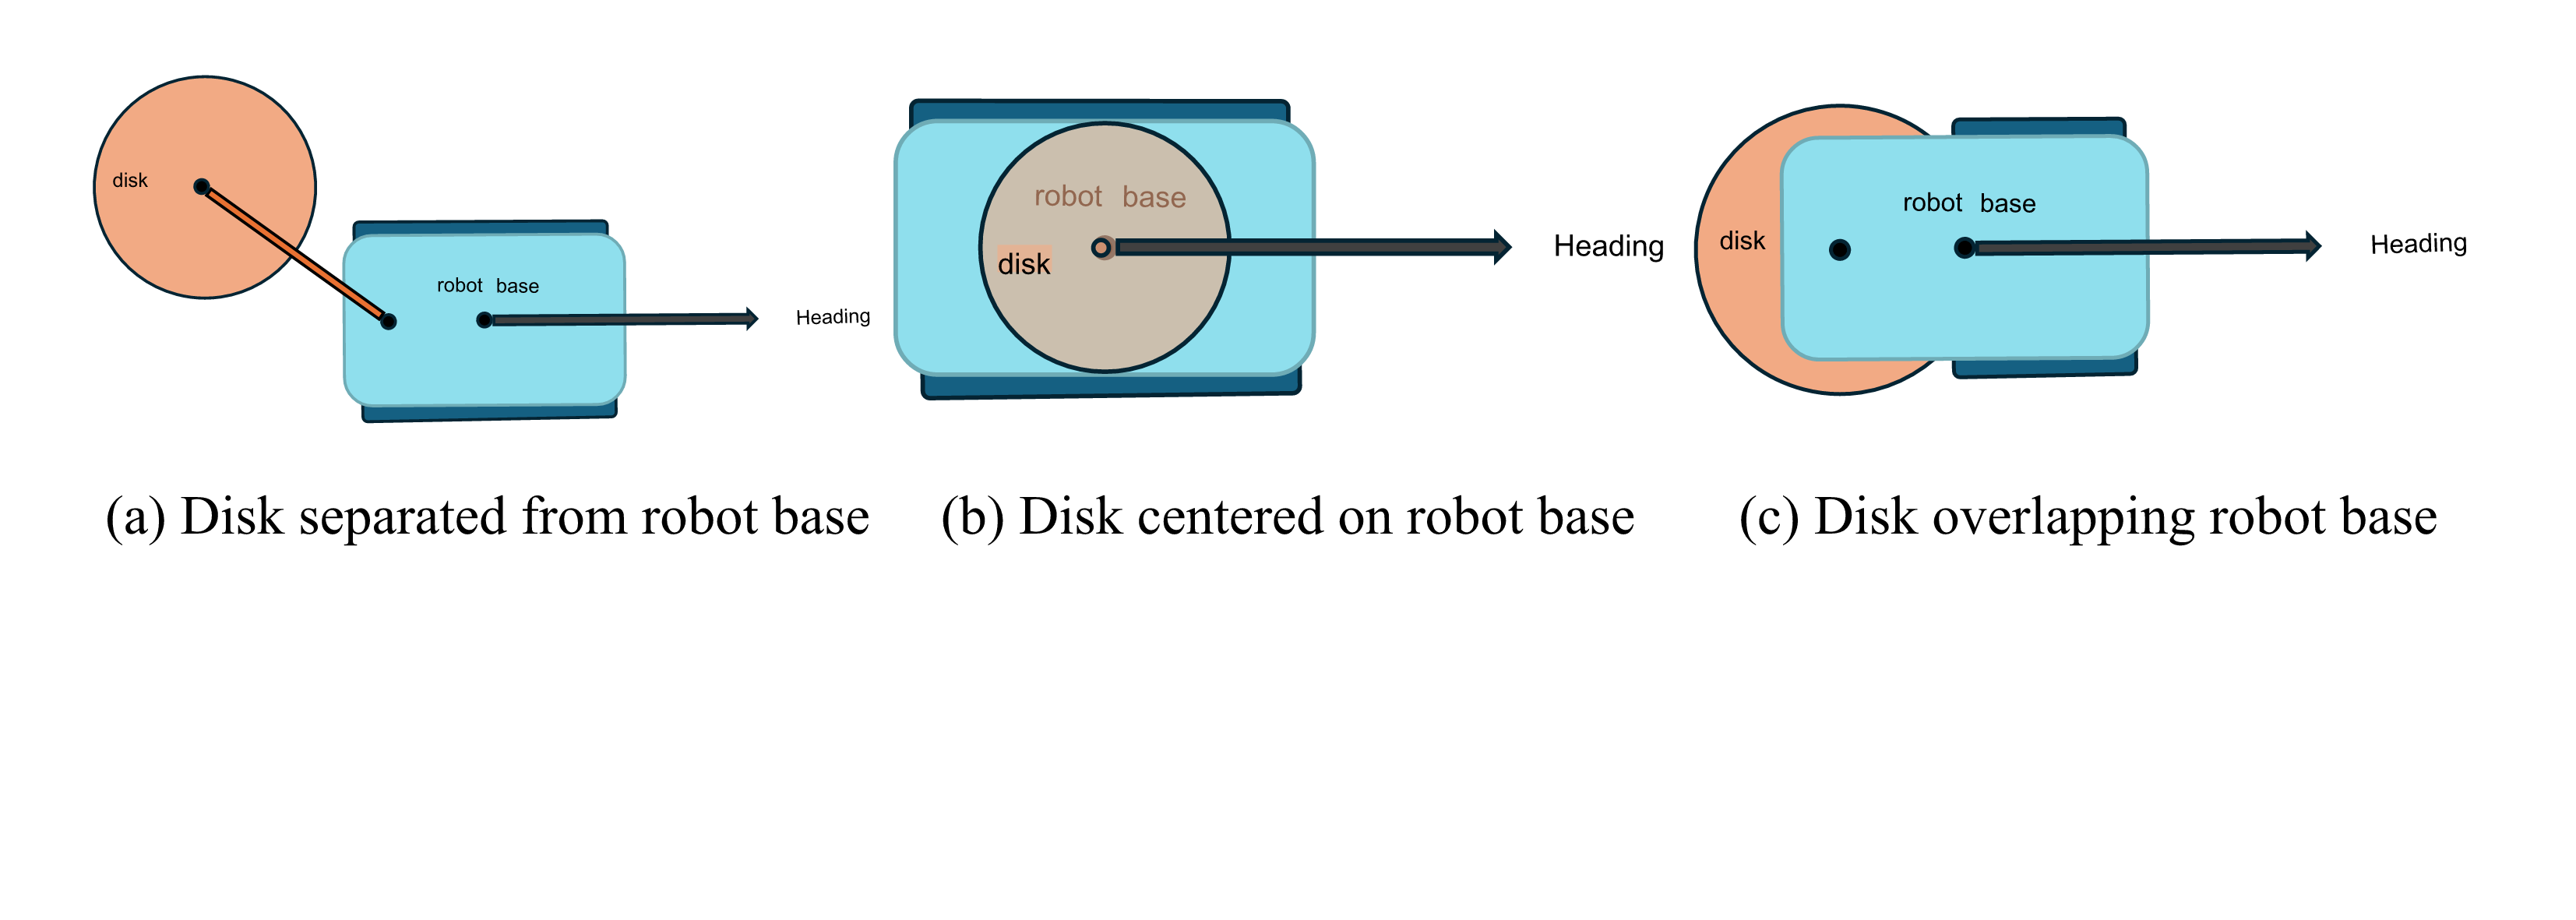
\includegraphics[width=0.98\linewidth]{figures/figure_2_disc_vehicle_relationships.png}
  \caption{三类抹盘与车体相对位置关系示意图。 (a) 前置抹盘；(b) 下置或中心抹盘；(c) 摆臂末端抹盘。箭头表示车体行驶方向，虚线表示工具覆盖或摆臂可达范围。}
\end{figure}
```

  

混凝土地面机器人研究经历了由机械化、遥控化向局部自主化发展的过程。早期系统主要以减轻人工负担为目标，通过轻量化底盘、抹平机构和遥控器完成大面积地面施工。Kobayashi 等人的系统覆盖木抹与金属抹工序，并通过真实工地试验验证了作业能力，但设备仍以无线遥控和示教复现为主，现场效果受到进入时机、地面摩擦和操作经验影响；其车轮转向还可能在新浇混凝土上留下难以消除的痕迹 [4]。Hwangbo 等人随后将现有骑乘式抹光机改造为无人平台，采用激光扫描与反射标志进行定位，并由基于施工图的任务规划器生成路线 [5]。该系统说明规则大空间内的自主抹平具有可行性，但其作业工具仍相对车体固定，覆盖模型更接近第二类固定足迹平台。

  

摆臂式机器人通过将抹盘安装在可转动的长臂末端扩展了上述平台的工作空间。相较于工具固定在车体下方或前方的构型，摆臂能够在车体保持安全距离时覆盖侧向区域，并通过改变摆角形成多种车体—工具相对姿态。这种运动冗余有利于覆盖墙边、柱边和窄通道入口，也可能减少车体在湿混凝土上的行驶与急转弯。然而，车体可通行并不意味着抹盘可作业，抹盘可达也不意味着车体、摆臂和抹盘整体无碰撞。规划必须同时判断车体矩形包络、摆臂线段或胶囊包络以及圆形抹盘与障碍物的关系，并在四维状态 $(x_c,y_c,\theta,\phi)$ 中组织连续运动 [6]。

  

目前最接近这一问题的 SatAOI 方法从障碍栅格出发，建立车体、摆臂与抹盘的几何模型和碰撞原则，并通过全局搜索识别摆臂机器人可进入、可作业且相互连通的区域 [6]。该工作解决了“哪里可以作业”的基础问题，却没有回答“以什么顺序、采用何种车体—摆臂运动完整覆盖这些区域”。因此，从 AOI 界定到可执行 CPP 之间仍缺少区域分解、全局访问、局部覆盖与速度协调等关键环节。

  

## 2.2 覆盖路径规划方法

  

关于现有 CPP 方法的讨论可以从“地图处理能力”和“机器人建模精度”两个角度看。地图处理能力指方法能否在含有多障碍、孔洞、狭窄连接和不规则边界的场景中稳定生成覆盖单元、邻接关系和转场路径；机器人建模精度指方法是否把机器人及工具作为具有尺寸、姿态、运动约束和碰撞关系的系统来处理，而不是只使用点、圆盘或固定宽度条带近似。由此可以得到四类方法：简单地图处理能力与粗略机器人建模、复杂地图处理能力与粗略机器人建模、简单地图处理能力与精细机器人建模，以及复杂地图处理能力与精细机器人建模。摆臂式抹平 CPP 需要落在第四类，因为施工地图通常被墙体、立柱和孔洞切割，而机器人覆盖足迹又由车体运动和主动摆臂共同决定。

  

第一类方法以经典覆盖算法为代表，能够清楚表达覆盖思想，但通常只在较理想的地图和简化机器人模型下闭合问题。BCD 根据扫描线连通关系变化切分区域，并在单元内生成 Boustrophedon 式往复扫掠 [9]；STC 在自由栅格图上构造生成树，并沿树边界形成系统遍历 [10]。二者分别说明了细胞分解和图遍历在 CPP 中的基本作用，但覆盖原语通常仍是点机器人、圆盘机器人或固定宽度工具。若直接用于摆臂抹平任务，这类方法无法判断车体、摆臂和抹盘之间的相对姿态，也无法描述摆角变化对瞬时覆盖足迹和碰撞风险的影响。

  

第二类方法具有较强的复杂地图处理能力，并已形成可复现的开源工程框架，但机器人和工具仍多被建模为固定足迹。ETH Zurich 的 `polygon_coverage_planning` 面向带孔一般多边形，采用 BCD 或梯形分解生成单元，为每个单元构造多个扫掠候选，并通过 Equality Generalized Traveling Salesman Problem 和可见图完成全局选择与避障转场 [11,12]。Fields2Cover 面向农业车辆，支持非凸场地、障碍物、地头、作业条带、路线排序以及 Dubins 或 Reeds–Shepp 型曲率受限连接 [13,14]。Nobleo Full Coverage Path Planner 在 ROS 占据栅格上实现 Backtracking Spiral Algorithm/Spiral-STC 类覆盖，并可分别配置机器人半径和工具半径 [15]。这些框架说明复杂边界、障碍和工程接口已经可以被系统处理；但其工具宽度、机具宽度或工具圆相对车体基本固定，不能表达摆臂角 $\phi$ 改变时抹盘位置连续变化所形成的时变扫掠。

  

第三类方法更重视机器人运动约束、可达性和碰撞关系，但地图任务通常不是复杂二维地面完整覆盖。Fields2Cover 中的非完整车辆连接已经考虑了最小转弯半径和车辆运动学 [13,14]，但它服务于固定机具宽度下的农业条带作业；移动机械臂表面覆盖研究能够显式处理底盘、机械臂、末端工具、可达性和遮挡，例如面向喷雾消毒的区域覆盖方法可从三维表面生成末端执行器轨迹，并联合选择移动底盘位置和机械臂运动 [17]。这类工作对“机器人如何执行”建模更细，却通常面向规则场地、农田条带或三维物体表面，而不是在已知二维施工地图中同时完成障碍处理、区域分解、全局遍历和连续地面覆盖评价。

  

第四类是本文所需的目标区域：既能处理复杂施工地图，又能精细保留摆臂机器人几何。SatAOI 是最接近这一方向的工作，它从障碍栅格出发，显式建立车体、摆臂与抹盘的几何模型和碰撞原则，并通过全局搜索识别摆臂机器人可进入、可作业且相互连通的区域 [6]。然而，SatAOI 解决的是“哪里可以作业”，并不生成“以什么顺序、通过何种局部车体—摆臂运动完成覆盖”的 CPP 结果。因此，在第四类中仍缺少从复杂地图到可执行覆盖轨迹的完整规划链条。本文方法即定位于这一缺口：在保留摆臂几何和速度约束的同时，将地图分区、连通修复、访问排序、局部摆扫和连续覆盖评价连接为统一流程。

  

表 1 按上述两个维度重新比较代表性方法。这里的“局限”专指将方法直接用于“移动车体 + 主动摆臂 + 圆形抹盘”任务时需要解决的问题，而不是对相关算法或软件总体性能的评价。

  

```{=tex}
\begingroup
\footnotesize
\renewcommand{\arraystretch}{1.18}
\setlength{\tabcolsep}{1pt}
\setlength{\LTleft}{0pt}
\setlength{\LTright}{0pt}
\begin{longtable}{@{}>{\RaggedRight\arraybackslash}p{0.115\textwidth}>{\RaggedRight\arraybackslash}p{0.16\textwidth}>{\RaggedRight\arraybackslash}p{0.17\textwidth}>{\RaggedRight\arraybackslash}p{0.235\textwidth}>{\RaggedRight\arraybackslash}p{0.295\textwidth}@{}}
\caption{代表性覆盖路径规划方法及其对摆臂抹平任务的适用性}\\
\toprule
方法 & 地图处理能力 & 机器人建模精度 & 覆盖及全局路线机制 & 用于本场景的主要局限 \\
\midrule
\endfirsthead
\multicolumn{5}{c}{\small 表 1（续）}\\
\toprule
方法 & 地图处理能力 & 机器人建模精度 & 覆盖及全局路线机制 & 用于本场景的主要局限 \\
\midrule
\endhead
\bottomrule
\endfoot
BCD \refjump{choset1998}{9} & 中等；可处理拓扑事件，但复杂孔洞会增加细碎单元 & 粗略；点或固定宽度工具 & 单元内平行往复扫掠；遍历单元邻接图 & 不包含摆臂状态，也不描述车体—摆臂协同覆盖 \\
STC \refjump{gabriely2001}{10} & 中等；可接入不规则占据栅格，但受分辨率和回溯影响 & 粗略；点、圆盘或固定工具足迹 & 沿栅格生成树系统遍历，必要时回溯 & 无法利用主动摆臂的时变可达范围，覆盖精度受栅格尺度限制 \\
polygon coverage planning \refjump{bahnemann2021}{11}, \refjump{polygoncoverage}{12} & 强；支持带孔多边形、分解候选和避障转场 & 粗略；固定扫线间距，主要面向飞行器覆盖 & 多扫掠候选 + Equality-GTSP；可见图转场 & 不能表示摆臂改变的瞬时足迹；候选组合规模随复杂度增大 \\
Fields2-\newline Cover \refjump{mier2023}{13}, \refjump{fields2cover}{14} & 强；支持非凸边界、障碍、地头和路线优化 & 中等；固定机具宽度 + 非完整车辆转弯约束 & 固定宽度条带、路线优化和曲率受限连接 & 地头假设与室内施工不同；固定条带无法表达车体—摆臂协同覆盖 \\
Nobleo FCPP \refjump{nobleo}{15} & 强；面向 ROS 占据栅格和室内导航接口 & 粗略到中等；机器人半径和工具半径可分设但相对位姿固定 & BSA/Spiral-STC 式覆盖并接入导航栈 & 没有主动摆臂自由度，无法协调摆角、摆速和车速 \\
移动机械臂表面覆盖 \refjump{thakar2022}{17} & 弱到中等；侧重三维表面或局部作业区域 & 强；显式考虑底盘、机械臂、末端工具和可达性 & 末端轨迹与底盘停靠位/机械臂运动联合规划 & 面向三维表面与剂量约束，不提供复杂二维地面的完整分解和连续遍历 \\
SatAOI \refjump{lin2025}{6} & 强；面向施工障碍栅格，可识别 AOI 与连通性 & 强；显式车体—摆臂—抹盘四维状态和碰撞关系 & 全局搜索与可作业区域判定，不生成完整覆盖路线 & 只界定 AOI 与连通性，未解决分区、访问排序和局部覆盖执行 \\
本文方法 & 强；以矩形候选、补洞和连通修复处理含障碍二维施工地图 & 强；保留车体、摆臂、抹盘几何及速度耦合 & 矩形分区、邻接修复、全局访问、局部摆扫和连续扫掠评价 & 采用启发式近似分区与访问排序，当前仍以已知静态二维地图为输入 \\
\end{longtable}
\endgroup
```

  

### 2.3 小结与研究缺口

  

上述比较表明，现有方法已经分别覆盖了复杂地图分解、固定足迹机器人的完整覆盖、非完整车辆的转弯连接、移动机械臂的末端可达，以及摆臂抹平机器人的 AOI(Area Of Interest) 界定。然而，若把目标限定为“已知复杂二维施工地图中的摆臂式抹平机器人完整覆盖”，仍存在三个与本文贡献一一对应的缺口。

  

**第一是机器人建模缺口。** 现有 CPP 的基本覆盖原语多为固定宽度条带或固定工具栅格，不能表达抹盘相对车体随 $\phi$ 连续变化的扫掠足迹。若简单以摆臂最大工作半径替代固定工具宽度，会把“几何上某一姿态可达”误当成“沿整条轨迹连续可覆盖”，也无法正确判断摆臂与障碍物的碰撞。对应地，本文在规划模型中显式保留车体、摆臂和圆形抹盘几何，并以连续轨迹的末端扫掠作为覆盖评价对象。

  

**第二是复杂地图与局部原语耦合的缺口。** 已有开源框架能够处理多边形孔洞、占据栅格或非凸场地，SatAOI 也可以识别摆臂机器人可作业区域及其连通性，但这些能力尚未与适合车体—摆臂协同摆扫的覆盖单元和访问路线统一起来。因而，几何上覆盖充分的分区可能形成多个无法连续访问的分量，而图上连通的分区也可能缺少可执行的局部运动。对应地，本文采用面向摆扫原语的矩形候选表示、补洞和连通性修复，在复杂障碍地图中同时服务于区域覆盖和连续访问。

  

**第三是速度权衡缺口。** 对固定工具而言，扫线间距可以在规划阶段直接设定；对摆臂工具而言，实际覆盖还取决于摆臂角速度、车速、转向时间和非作业转场。只输出无时间参数的中心线，无法判断圆盘扫掠是否留有空隙，也不能公平评价覆盖率与总工期的权衡。对应地，本文在局部覆盖原语和实验评价中引入车体线速度 $v$ 与摆臂角速度 $\omega_a$ 的匹配关系，用覆盖率、执行时长和单位覆盖面积耗时共同描述这一 trade-off。

  

因此，本文聚焦的研究缺口是：在已知、含密集障碍的二维施工环境中，尚缺少一种以摆臂动态足迹为核心，同时连接区域表示、遍历连通性、全局访问、局部车体—摆臂协调和连续扫掠评价的端到端 CPP 方法。本文后续提出的矩形候选分区并非经典 BCD 的替代性精确分解，而是一种面向摆臂运动原语的近似区域表示；其目标是在明确适用边界的前提下，补全从 AOI 到可执行覆盖轨迹的规划链条。
